\newpage
\section{Introduction}
\newcommand{\AWstar}{$\mathrm{AW}[\star]$}



Instead of solving a single algorithmic problem, \emph{algorithmic meta-theorems} 
establish the tractability of whole classes of problems, in a uniform way.
The targeted problem class is commonly defined using logic, and hence many algorithmic meta-theorems fit the following template.

\newcommand{\placeholder}[1]{\textup{\textbf{$\boldsymbol{\langle}$#1$\boldsymbol{\rangle}$}}}
\begin{quote}
\emph{Every problem expressible in \placeholder{logic} can be solved in time \placeholder{runtime} on every input satisfying \placeholder{tameness condition}.}
\end{quote}
%
A prototypical example is Courcelle's Theorem, which states that every problem definable in \emph{monadic second-order logic} is solvable in \emph{linear time} on graphs with constant \emph{tree-width}~\cite{courcelle1990monadic}.
Similarly, a result of Frick and Grohe
implies that every graph problem definable in \emph{first-order logic} (FO) can be decided in \emph{linear time} on all \emph{planar graphs}~\cite{frick2001deciding}.
In particular, the \emph{(first-order) model checking problem} 
-- does a given graph $G$ satisfy a given FO sentence $\phi$?  -- is \emph{fixed-parameter tractable}~(fpt) on planar graphs. 
That is, it is solvable\footnote{Throughout this paper, we use the uniform -- but not strongly uniform -- version of fpt, and of fpt reductions. That means that the function $f$ need not be computable, but there is a single algorithm which solves the problem, independent of the parameter ($\phi$ in the case of model checking).} in time $f(|\phi|)\cdot |V(G)|^c$, for some function $f$ and constant~$c$ (with $c=1$ in this specific case).
Many natural graph problems are expressible in FO.
For example, the sentence
\[
    \exists x_1 \ldots \exists x_k  \forall y\ 
    \bigvee_i\big(E(y,x_i) \vee (y = x_i)\big)
\]
expresses $k$-\textsc{Dominating-Set}: the existence of $k$ vertices  such that every vertex is either adjacent or equal to at least one of them.
Further expressible problems include $k$-\textsc{Independent-Set}, $k$-\textsc{Clique}, and $H$-\textsc{Subgraph-Isomorphism}.
With no further restrictions made on the input graphs,
these problems appear to be highly intractable.
Indeed, model checking on general graphs is believed not to be fpt; this is equivalent to the $\mathrm{FPT}{\neq}\mathrm{AW}[\star]$ conjecture.
This raises the question -- first posed by Grohe~\cite[Section~8.2]{logic-graphs-algorithms} -- on which graph classes\footnote{A \emph{graph class} is a (usually infinite) set of graphs.} 
the problem becomes fpt.
After decades of research, \emph{monadic dependence} has crystallized as the conjectured tractability limit for \emph{hereditary}\footnote{A graph class is \emph{hereditary} if it is closed under taking induced subgraphs, i.e., deleting vertices.} classes (see, e.g.,~\cite{warwick-problems,new-perspective-journal,tww4,ms-mc1}).

\begin{mcconjecture}\label{conj:main2}
  A hereditary graph class admits fixed-parameter tractable first-order model checking if and only if it is monadically dependent (assuming $\mathrm{FPT}{\neq}\mathrm{AW}[\star]$).
\end{mcconjecture}


  
Monadic dependence is a model-theoretic tameness notion that originates in Shelah's classification theory~\cite{BS1985monadic}.
It subsumes many tameness notions from structural graph theory, such as planarity, excluding a minor, bounded degree, bounded expansion, nowhere denseness, and bounded clique-width, twin-width, and merge-width.
See \Cref{fig:hierarchy} for a hierarchy of included graph classes.
For hereditary graph classes, monadic dependence is characterized as follows~\cite{flip-breakability}.
A hereditary graph class $\CC$ is \emph{monadically independent} if there is some formula $\phi(x,y)$ with the following property: for every graph \(H\) there is some graph $G \in \CC$ 
such that $H$ is an induced subgraph of the graph with vertices $V(G)$ and edges \(\{ uv \,:\, \text{ $\phi(u,v)$ or $\phi(v,u)$ holds in $G$} \}\).
Intuitively, this means that every graph can be encoded by $\phi$ in $\CC$.
Then $\CC$ is \emph{monadically dependent} if it is not monadically independent.

\medskip
In a previous paper~\cite{flip-breakability} we resolved the hardness direction of the Model Checking Conjecture, by showing that model checking is 
\AWstar-hard on every hereditary graph class that is not monadically dependent.

\subsection{Our results}
In this paper, we confirm the Model Checking Conjecture by proving its tractability direction.

% lax begin Lax185574.ModelChecking
\begin{restatable}{theorem}{mainthm}\label{thm:main}
  There is an algorithm which
  solves the model checking problem for first-order logic on graphs --
  does a given graph $G$ satisfy a given first-order sentence $\phi$?  -- with the following guarantee.
  For every monadically dependent graph class $\CC$ and real $\eps>0$, the algorithm runs in time $O_{\CC,\phi,\eps}(n^{3+\eps})$ for $n$-vertex graphs $G\in\CC$.
\end{restatable}
% lax end

In particular, this gives fpt first-order model checking on all classes of bounded twin-width and bounded merge-width, without requiring a decomposition as part of the input. 

We remark that our algorithm is uniform:
it takes both $G$ and $\phi$ as input, and does not depend on the graph class $\CC$, which only appears in the running-time guarantee.
Our result lifts from graphs to monadically dependent classes of binary structures -- structures over a fixed signature consisting of binary relation symbols -- using a standard encoding (see, e.g., Lemma~19.11 in the full version of~\cite{flip-breakability}).



\medskip
Our algorithm is based on dynamic programming on graph decompositions called \emph{construction sequences} of \emph{almost bounded merge-width}.
In a companion paper with Michał Pilipczuk~\cite{md-abmw}, we prove that they exist and can be computed efficiently on monadically dependent graph classes.

Existing model checking algorithms for classes of bounded twin- or merge-width have a tower-of-exponentials dependence on the width. This prevents their direct application to decompositions of \emph{almost} bounded merge-width, where the width is only bounded by a subpolynomial function $n^{o(1)}$ of the input size $n$, rather than a constant. 
To overcome this obstacle, we make the running time depend on the number of \emph{types} that are realized in the graph. We control this number using a type-counting result for monadically dependent classes, which we believe to be of independent interest.

This result provides polynomial bounds on the number of quantifier rank $q$ types $\tp_q^G(\tup v/U)$ of $k$-tuples $\tup v$ over a set $U$ of parameters.
The \emph{type} $\tp_q^G(\tup v/U)$ is the set of formulas of quantifier rank at most \(q\), with parameters from \(U\), which hold of the tuple $\tup v$ in $G$
(see \Cref{sec:prelims} for the precise definition).
For $q=0$, the type $\tp_0^G(v/U)$ of a vertex $v\notin U$ represents its neighborhood $N(v)\cap U$ in $U$. 
In general graphs, there could be $2^{|U|}$ many such neighborhoods, but the fundamental Sauer--Shelah lemma~\cite{Sauer72,She72} bounds their number by $(|U|+1)^d$, where $d$ is the VC-dimension of the graph $G$.
The VC-dimension $d$ is bounded uniformly in every monadically dependent class.
For $q=1$, the type $\tp_1^G(v/U)$ of a vertex $v$ 
determines $\setof{N(w)\cap U}{w\in N(v)}$, the set of neighborhoods in $U$ of the neighbors of $v$. In general graphs there could be 
$2^{2^{|U|}}$ many such sets, and so on for higher $q$: the number of $q$-types over a set $U$ can reach a tower of height $q+1$.
The following result, which is the cornerstone of our approach, can thus be seen as an extension of the Sauer--Shelah lemma to higher quantifier ranks, in monadically dependent graph classes.


% lax begin Lax185574.TypeBound
\begin{theorem}[{Simplified form of \Cref{thm:type-bound}}]\label{thm:intro-type-bound}
Let $\CC$ be a monadically dependent graph class and $k,q\in\N$. There is some $d\in\N$ such that for every (possibly infinite) graph $G \in \CC$,  and finite subset $U \subseteq V(G)$ with $|U|>1$
we have
\[
  \left|
    \{\tp^{G}_q(\tup v/U) \,:\, \tup v \in V(G)^k \}\right|
    \leq  |U|^d.
\]
\end{theorem}
% lax end

\Cref{thm:intro-type-bound} is a finitary analogue of a fundamental result in stability theory due to Shelah~\cite{Shelah1969}, which bounds the number of complete types (of unbounded quantifier rank) over an infinite set $U$, by $|U|^\kappa$ in every \emph{stable} class of structures, for some cardinal $\kappa$ depending on the class. 
Its proof blends ideas from \cite{number-of-types} and \cite{flippers}.

\medskip
A technical overview of the proofs of the main results is presented in \Cref{sec:tech-overview}. 
All our results are formalized in Lean. At \url{https://laxarchive.org/lax-185574/}, each definition, lemma, and theorem is annotated with its proven Lean counterpart.


\begin{figure}[htb]
  \centering
  % Three columns (sparse notions | stable dense notions | dependent dense notions) and
% four rows. Arrows are implications. All properties in the same row are equivalent
% on weakly sparse classes. Unlike the original, tree-depth and shrub-depth are left out.
%
% Where model checking is known to be fpt, one centered line below the name of the
% property (\mcdec) cites the algorithm (labeled mc), which assumes a suitable
% decomposition of the input graph to be given, and an algorithm computing such a
% decomposition, or says that this is open (labeled dec). For nowhere denseness both
% are in the same paper, which the line cites once (\mcanddec, labeled mc+dec), and
% for monadic dependence model checking is this paper.
% Bounded stable merge-width coincides with structurally bounded expansion, so its box
% cites the algorithms for the latter: model checking given a decomposition, and the
% efficient reversal of transductions that computes one. The line is gray, including
% the link color, so that it does not distract from the names of the properties.
%
% The bottom line of a box (\ex, gray italics) names example graph classes for which
% this box is the most restrictive property in the hierarchy that they have, each
% followed by a citation (\excite, upright and gray including the link color, like the
% citations of the box itself) of an fpt model checking algorithm for that class.
%
% Boxes are \bw wide and \bh high, the columns are \cs apart (center to center) and
% the rows \rs apart. Each box has three bands: the label on a light gray background,
% the citations on a lighter gray one, and the examples on white. The label band takes
% the top half of the box, and the other two bands a quarter each. A black rule \hz
% below the top of the box separates the label from the citations, and the citations
% end \fz above the bottom, at a gray rule of the same width. The label is centered \tz
% below the top, in the middle of the space above the rule. It is set in a tabular, whose struts align the baselines
% of the one-line labels and center the two-line ones at the same height.
% The baselines of the citations and of the examples are \rb and \eb above the bottom
% of the box. The bands and the rules are drawn in the path picture of the box, which
% comes before its border, so the border lies on top of them. Arrows within a row join
% the boxes at the height of the labels, so that they do not continue the black rules.
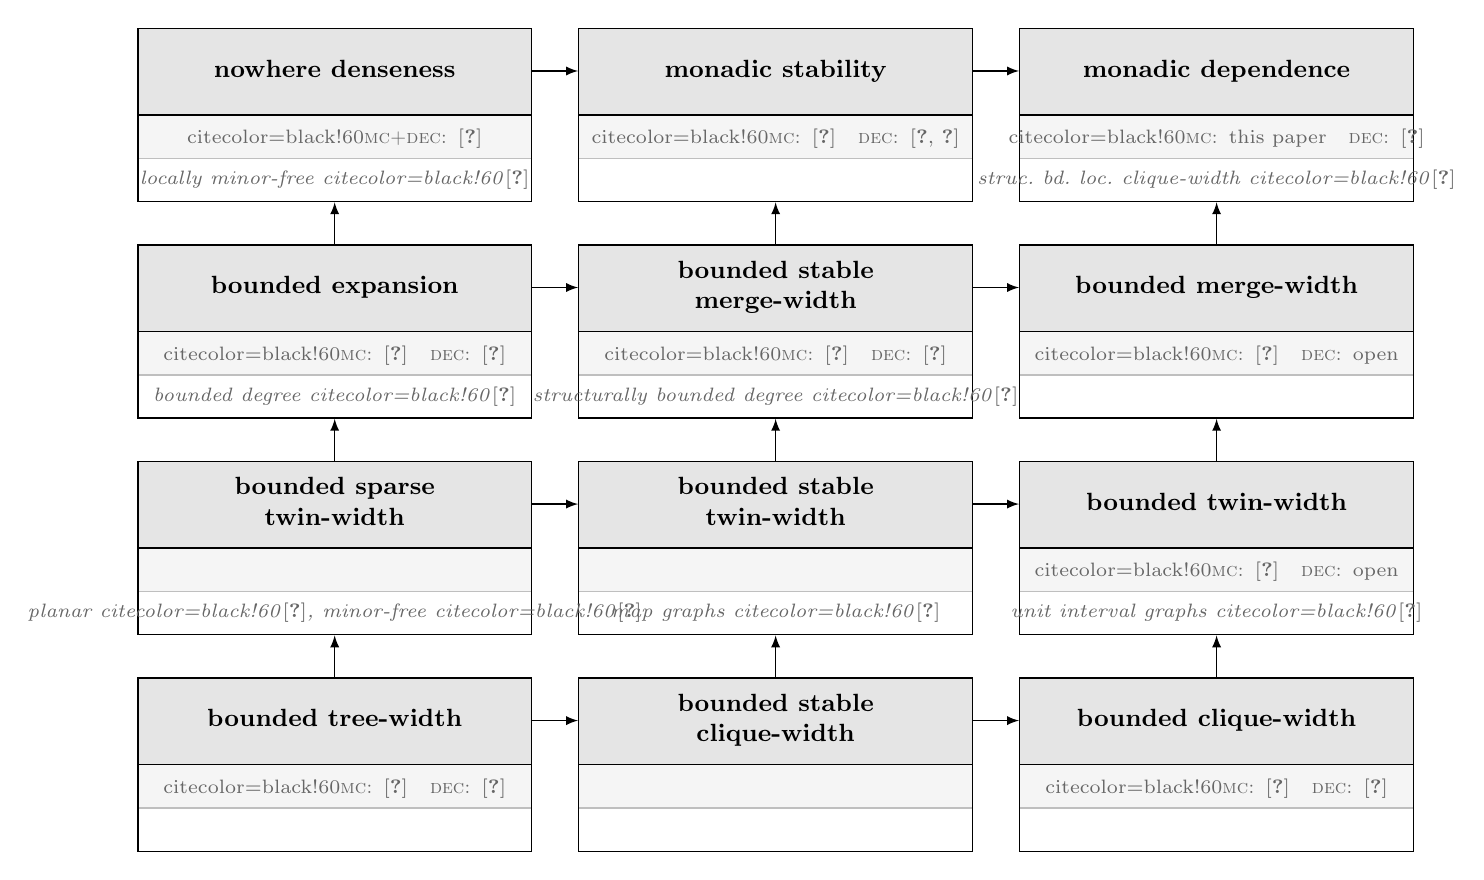
\begin{tikzpicture}[
        prop/.style={draw, line width=0.5pt, minimum width=\bw, minimum height=\bh,
            path picture={\def\pb{path picture bounding box}
                \fill[black!10] (\pb.north west) rectangle ([yshift=-\hz]\pb.north east);
                \fill[black!4] ([yshift=-\hz]\pb.north west) rectangle ([yshift=\fz]\pb.south east);
                \draw[head] ([yshift=-\hz]\pb.north west) -- ([yshift=-\hz]\pb.north east);
                \draw[foot] ([yshift=\fz]\pb.south west) -- ([yshift=\fz]\pb.south east);}},
        proplabel/.style={font=\small\bfseries, inner sep=0pt},
        imp/.style={line width=0.5pt, -latex},
        detail/.style={inner sep=0pt, anchor=base, font=\scriptsize},
        refs/.style={detail, text=black!60,
            execute at begin node={\hypersetup{citecolor=black!60}}},
        example/.style={detail, font=\scriptsize\itshape, text=black!60},
        head/.style={line width=0.5pt},
        foot/.style={line width=0.5pt, black!25},
    ]
    \def\bw{5.0cm}\def\bh{2.2cm}\def\cs{5.6}\def\rs{2.75}
    \def\tz{0.55cm}\def\rb{0.745cm}\def\fz{0.55cm}\def\eb{0.225cm}\def\hz{1.1cm}
    \def\prop#1#2#3{\node[prop] (#1) at (#2) {};
        \node[proplabel] at ([yshift=-\tz]#1.north) {\begin{tabular}{@{}c@{}}#3\end{tabular}};}
    \def\lbl#1{\textsc{#1}}
    \def\mcdec#1#2#3{\node[refs] at ([yshift=\rb]#1.south)
        {\lbl{mc:}\enspace#2\quad\lbl{dec:}\enspace#3};}
    \def\mcanddec#1#2{\node[refs] at ([yshift=\rb]#1.south) {\lbl{mc+dec:}\enspace#2};}
    \def\ex#1#2{\node[example] at ([yshift=\eb]#1.south) {#2};}
    \def\excite#1{{\hypersetup{citecolor=black!60}\textup{\cite{#1}}}}

    % sparse notions
    \prop{nd}{0,0}{nowhere denseness}
    \prop{be}{0,-\rs}{bounded expansion}
    \prop{sptw}{0,-2*\rs}{bounded sparse\\twin-width}
    \prop{trw}{0,-3*\rs}{bounded tree-width}

    % stable dense notions
    \prop{ms}{\cs,0}{monadic stability}
    \prop{smw}{\cs,-\rs}{bounded stable\\merge-width}
    \prop{stw}{\cs,-2*\rs}{bounded stable\\twin-width}
    \prop{scw}{\cs,-3*\rs}{bounded stable\\clique-width}

    % dependent dense notions
    \prop{md}{2*\cs,0}{monadic dependence}
    \prop{mw}{2*\cs,-\rs}{bounded merge-width}
    \prop{tww}{2*\cs,-2*\rs}{bounded twin-width}
    \prop{cw}{2*\cs,-3*\rs}{bounded clique-width}

    % fpt model checking, and computing the decompositions it needs
    \mcanddec{nd}{\cite{gks}}
    \mcdec{be}{\cite{DvorakKT13-journal}}{\cite{grad-and-bounded-expansion-Nesetril}}
    \mcdec{trw}{\cite{courcelle1990monadic}}{\cite{minorsXIII}}
    \mcdec{ms}{\cite{ms-mc1}}{\cite{flippers,ms-mc2}}
    \mcdec{md}{this paper}{\cite{md-abmw}}
    \mcdec{smw}{\cite{lsd-journal}}{\cite{dreier2026efficient}}
    \mcdec{mw}{\cite{mw-stoc}}{open}
    \mcdec{tww}{\cite{tww1}}{open}
    \mcdec{cw}{\cite{courcelle2000linear}}{\cite{OumSeymour-approximating}}

    % example graph classes
    \ex{sptw}{planar~\excite{frick2001deciding}, minor-free~\excite{flum2001fixed}}
    \ex{be}{bounded degree~\excite{seese_1996}}
    \ex{smw}{structurally bounded degree~\excite{new-perspective-journal}}
    \ex{stw}{map graphs~\excite{eickmeyer2017map}}
    \ex{tww}{unit interval graphs~\excite{ganian2015fo}}
    \ex{md}{struc.\ bd.\ loc.\ clique-width~\excite{DBLP:conf/lics/BonnetDGKMST22}}
    \ex{nd}{locally minor-free~\excite{dawar2007locally}}

    % implications within the columns
    \foreach \a/\b in {trw/sptw, sptw/be, be/nd,
                       scw/stw, stw/smw, smw/ms,
                       cw/tww, tww/mw, mw/md}
        \draw[imp] (\a) -- (\b);

    % implications within the rows
    \foreach \a/\b in {nd/ms, ms/md, be/smw, smw/mw, sptw/stw, stw/tww,
                       trw/scw, scw/cw}
        \draw[imp] ([yshift=-\tz]\a.north east) -- ([yshift=-\tz]\b.north west);
\end{tikzpicture}%

  \caption{A hierarchy of graph class properties that admit fpt first-order model checking.
    Arrows represent implications between properties.
    In particular, \emph{bounded tree-width} is the most restricted class property in this hierarchy and \emph{monadic dependence} is the most general one.
    In each box where applicable, \textsc{mc} cites the fpt model checking result which assumes a suitable decomposition is given, while \textsc{dec} cites the result providing such decompositions efficiently; \textsc{dec:}~open means that no algorithm for computing such a decomposition is known.
    Example graph classes are listed in \textcolor{black!60}{\emph{italics}}, each under the most restricted property that subsumes it, together with a citation to an fpt model checking algorithm for that class.}
  \label{fig:hierarchy}
\end{figure}

\subsection{Related work}
\Cref{thm:main} completes a long line of research on first-order model checking on hereditary graph classes.
An overview of previous model checking results is given in \Cref{fig:hierarchy}. 
In particular, the Model Checking Conjecture was previously known to hold in the following three settings, which we discuss below:

\newcommand{\footnoteMonotone}{\footnote{A graph class is \emph{monotone} if it is closed under taking subgraphs, i.e., deleting vertices and edges.}}
\newcommand{\footnoteEdgeStable}{\footnote{\interlinepenalty=10000 % keep this footnote on one page
A graph class is \emph{edge-stable} if it excludes some semi-induced half-graph, i.e., there is $k\in\N$ such that no graph in the class contains vertices $a_1,\ldots,a_k,b_1,\ldots,b_k$ where $a_i$ and $b_j$ are adjacent if and only if $i\le j$. Equivalently, the edge relation is a stable formula on the class in the sense of model theory.}}
\newcommand{\footnoteOrdered}{\footnote{An \emph{ordered graph} is a graph equipped with a total order on its vertex set, which formulas can access via an additional binary relation symbol~$<$.}}

\begin{itemize}
  \item in \emph{monotone}\footnoteMonotone~graph classes,
  \hfill \cite{gks}

  where monadic dependence coincides with \emph{nowhere denseness};\hfill \cite{AdlerA14,podewski1978stable}
  
  
  \item in \emph{edge-stable}\footnoteEdgeStable~graph classes,
  \hfill \cite{ms-mc1,ms-mc2}

  where monadic dependence coincides with \emph{monadic stability};
  \hfill \cite{rankwidth-meets-stability}
  
  
  \item in classes of \emph{ordered graphs}\footnoteOrdered,
  \hfill \cite{tww4,tww1}

  where monadic dependence coincides with \emph{bounded twin-width}.
  \hfill \cite{tww4}
\end{itemize}

\paragraph*{Sparsity.}
The first model checking result in the sparse regime is the seminal Courcelle's Theorem, which established tractability for more expressive monadic second-order logic on all classes of bounded tree-width~\cite{courcelle1990monadic}.
Subsequently, Seese initiated the study of first-order model checking by showing tractability on all classes of bounded degree~\cite{seese_1996}.
This research direction gained momentum through the work of Grohe and his coauthors~\cite{frick2001deciding,flum2001fixed,dawar2007locally}; see Grohe's 2007 survey~\cite{logic-graphs-algorithms} for an account of these early developments.
This line of research (see also~\cite{dawar2009domination,DvorakKT13-journal,GroheKreutzer2011}) culminated in the model checking algorithm of Grohe, Kreutzer, and Siebertz~\cite{gks} for \emph{nowhere dense} classes.
This notion is one of the cornerstones of the \emph{sparsity theory} by \Nesetril and Ossona de Mendez~\cite{NesetrilM11a,sparsity-book} that shaped the field.
For monotone classes, this result is tight: first-order model checking is \AWstar-hard on every monotone class that is not nowhere dense~\cite{DvorakKT13-journal,dawar2009parameterized}.

\medskip
With the sparse classes resolved, the research focus has shifted towards possibly dense classes,
and two parallel research directions emerged.

\paragraph*{Stability.}
One research direction aims to lift the theory of nowhere dense classes to dense graphs.
Here a key notion is that of \emph{monadic stability}, a restriction of monadic dependence that also originates in model theory~\cite{BS1985monadic}.
The study of the model checking problem has revealed multiple new characterizations of monadic stability, such as \emph{flip-flatness}~\cite{dreier2023indiscernibles}, \emph{flipper games}~\cite{flippers}, and \emph{low shrub-depth covers}~\cite{horizons}.
They subsequently led to an fpt algorithm for first-order model checking for monadically stable classes~\cite{ms-mc1,ms-mc2}.
This result is tight in hereditary classes that are additionally edge-stable~\cite{ms-mc2,rankwidth-meets-stability}.
The ideas from this line of research have been further developed into combinatorial characterizations of monadically dependent graph classes such as \emph{flip-breakability}~\cite{flip-breakability} and \emph{flip-separability}~\cite{bonnet2025separability-icalp}.
This also includes the characterization by forbidden induced subgraphs, which settled the hardness part of the Model Checking Conjecture for all hereditary graph classes~\cite{flip-breakability}.


\paragraph*{Clique-width, twin-width, and merge-width.}
A second, parallel line of research has pushed the tractability frontier of first-order model checking through the development of new graph decompositions, often accompanied by new graph width parameters.
Mirroring tree-width in the sparse setting, it was shown early on by Courcelle, Makowsky, and Rotics that also classes of bounded \emph{clique-width} admit fpt monadic second-order model checking~\cite{courcelle2000linear}.

Twenty years later, inspired by the work of Guillemot and Marx on the permutation pattern problem~\cite{guillemot2014finding}, Bonnet, Kim, Thomass\'e, and Watrigant introduced the more general classes of bounded \emph{twin-width}, and showed that they admit fpt first-order model checking~\cite{tww1}.
Their algorithm is conditional in the sense that it requires as an additional input a decomposition witnessing the twin-width bound.
As of today it is not known how to efficiently compute or approximate these decompositions in general graphs. However, they can be efficiently approximated in many specific cases of interest~\cite{tww8}, in particular, in hereditary classes of ordered graphs~\cite{tww4}.
There, bounded twin-width forms the exact tractability limit for first-order model checking.

Inspired by twin-width and the related flip-width parameters~\cite{flip-width},
Dreier and Toru\'nczyk introduced \emph{merge-width}, a family of graph parameters based on decompositions called \emph{construction sequences}~\cite{mw-stoc}. 
A class has \emph{bounded merge-width} if for every radius $r$, every graph in the class has a construction sequence of radius-$r$ width bounded by a constant.
Again, those classes admit fpt first-order model checking under the condition that a construction sequence is given.
Crucial to our paper is the following relaxation of merge-width, called \emph{almost bounded merge-width}, which replaces the constant bound on the radius-$r$ width by $n^{o(1)}$, where $n$ is the vertex count of the graph. 
Dreier and Toru\'nczyk proved that hereditary classes of almost bounded merge-width are monadically dependent, and conjectured the converse~\cite{mw-stoc}.
The converse was first confirmed for radius one~\cite{neighborhood-complexity-mw}, and then in full~\cite{md-abmw}.
The proof of~\cite{md-abmw} is algorithmic: given a graph from a monadically dependent class, it computes in polynomial time a construction sequence of radius-$r$ width $n^{o(1)}$, for every fixed $r$.
Construction sequences of almost bounded merge-width form the basis for our model checking algorithm.

Note that it remains an open question how to approximate decompositions of constant width for classes with constant twin- and merge-width.
Thus, up until now and even in the light of \cite{md-abmw}, the previous model checking results for classes of bounded twin- and merge-width have remained conditional.
Therefore, our new algorithm marks the first time that unconditional model checking for all classes of bounded twin- and merge-width is established.





